\documentclass[12pt, letterpaper, onecolumn]{article}


\usepackage[utf8]{inputenc}

\usepackage{graphicx}
\usepackage{url}
% \usepackage{hyperref}
% \usepackage{anysize}
% \marginsize{2cm}{2cm}{1cm}{1cm}
% \usepackage[small,bf]{caption}
% Paquetes de la AMS:
\usepackage{amsmath, amsthm, amsfonts}

\usepackage{url}
\usepackage[bookmarksnumbered,pdfpagelabels=true,plainpages=false,colorlinks=true,
            linkcolor=black,citecolor=blue,urlcolor=blue]{hyperref}
\usepackage[margin=0.3in,labelfont=bf,labelsep=none]{caption}

\setlength{\textheight}{22.86cm}
\setlength{\textwidth}{15.24cm}
\setlength{\oddsidemargin}{.635cm}
\setlength{\topmargin}{-1.27cm}  

\usepackage[portuguese]{babel}

\usepackage{fancyhdr}
\pagestyle{plain}
\fancyfoot[CO,CE]{Confidential}
\fancyfoot[RO, LE] {\bf IME - USP}
\renewcommand{\headrulewidth}{0.4pt}
\renewcommand{\footrulewidth}{0.4pt}
\pagestyle{headings}
\setcounter{page}{1}


\title{\bf \huge Rede Social da Empresa Monashess Capital}
\author{{\bf Universidade de São Paulo} \\ {\bf Instituto de Matemática e Estatistica} \\ {\bf  \large Laborátorio de Programação Extrema} \vspace{1cm}\\{
\bf  \large Responsável: }\\ Camila Ferreira: \\cferreria at monashees dot com dot br}
\date{Julho de 2014}
\begin{document}

\maketitle
\begin{center}

\includegraphics[scale=.475]{images/ime.jpg}\hfil

\includegraphics[scale=2.25]{images/ccsl.png}\hfil

\includegraphics[scale=1]{images/logo.png}

\end{center}

\newpage
\tableofcontents
\newpage
% This sets section-numbering to only include Section and Subsection numbers
% \setcounter{secnumdepth}{2}



\section{Introdução} 
Monashees é uma empresa de venture capital que faz parcerias com empreendedores de destaque para construir grandes empresas. Esta empresa tem uma abordagem de longo prazo baseado na interação de seus sócios e empregados, mantendo um modelo de negócio adaptado ao ambiente brasileiro. \\

Monashees tem parcerias com empreendedores de alto impacto para construir grandes empresas, permitindo alavancar a a experiência coletiva, conhecimento e rede para completar suas equipes, definir a estratégia, ir ao mercado e planejar rodadas de financiamento adicionais. Além disso, essa parceria a longo prazo significa construir confiança e governança adequada.\\

A rede Plus Network foi construida com a finalidade de permitir a interação e colaboração de consultores e membros das startups do portfólio da Monashees, criando uma rede social em que empreendedores de Startups possam compartilhar ideias, pedir sugestões, etc. A ideia é ter uma comunidade de empreendedores altamente conectada e engajada. O importante é que empresas possam crescer juntas de uma forma mais estruturada. Pessoas podem encontrar outras pessoas no conjunto de empresas de acordo com especialidades específicas para começar alguma conversa ou observar posts relacionados. Gerenciamento de eventos por área, tema ou empresa. Pode existir um compartilhamento de arquivos por entre empresas. Impacto de 29 empresas no portfólio. Mais de dois mil usuários.\\

A Plus Network foi construída sobre o motor de desenvolvimento para redes sociais chamado ELGG.



\section{ELGG}
Elgg\footnote{ELGG: Motor para redes sociais de software livre - \url{http://elgg.org/}} é um software de código aberto para criação de redes sociais. Ele oferece um espaço de compartilhamento de informação e dados por intermédio de blog e micro-blogging, comunidades com fóruns de discussões ou blogs comunitários, espaço para repositório de arquivos, e-portfólio, tecnologia RSS para o conteúdo gerado dentro da rede, entre outras coisas. Todo conteúdo colocado no espaço pelos membros da rede social pode ser controlado por restrições de acesso e tudo pode ser catalogado por categorias, grupos e/ou palavras-chaves. Demo: \url{http://demo.elgg.org/}\\

O principal motivo da escolha do ELGG é o suporte pela comunidade por ser um motor de desenvolvimento de redes sociais de software livre. Outro motivo da escolha do ELGG ao invés do Noosfero foi a rapidez para colocar em Internet o projeto sem muitos privilégios sobre o sistema. Só foi instalar Mysql como servidor de banco de dados, apache como servidor web e os pacotes necessários para o desenvolvimento em PHP.

\subsection{Requerimento e instalação do Sistema} 
Durante o desenvolvimento do sistema, ele foi foi executado sobre Debian 7, Ubuntu 12.04 e Ubuntu 13.10. Como requerimentos para a configuração do ambiente de execução devem ser instaladas as seguintes aplicações:
\begin{itemize}
\item apache2
\item MySQL5+
\item PHP 5.2+
\item php5-curl (para o LinkedIn)
\item php5-gd 
\item php5-mysql 
\item php5-mcrypt
\item phpmyadmin
\end{itemize}

Desse modo, para instalação do ambiente de desenvolvimento, baixe o código da rede social do repositório, fazendo o clone do projeto no github (github.com/marcosamaris/labxp2014) sobre a pasta configurada para o servidor apache. No caso, por padrão, o diretório é {\texttt /var/www/}. Após baixar o código e demais informação do projeto, tem que criar uma pasta chamada startup-data sobre o mesmo nível da pasta startup. Esta pasta deve ter todos as permissões possíveis do sistema, ou seja que deve executar o comando {\texttt sudo chmod 777 -R startup-data} sobre o nível onde se encontra a pasta ou dar a permissão total ao usuário do apache (www-data).\\

Supondo que tenha o phpmyadmin instalado, deve adicionar phpmyadmin ao apache, para isso execute os seguintes comando, abra o arquivo {\texttt /etc/apache2/apache2.conf} e adicione no final do arquivo as seguinte linha: {\it include /etc/phpmyadmin/apache.conf}. Outra opção é baixar os arquivos do phpmyadmin e adicioná-los à pasta www do apache.\\

Ao final  reinicie seu servidor apache.\\
   
No seu navegador de internet, acesse o link: localhost/phpmyadmin. Faça o login no seu banco de dados com acesso root. Crie um usuário do banco com os seguintes dados:\\
        usarname: {\bf startup}\\
        password: {\bf monashees}\\

Faça logout com a conta root, e faça login com a conta recém criada, startup. Crie um novo banco de dados, cujo nome também será startup. Após a criação do banco, selecione ele, vá em importar e busque pelo banco.sql mais atualizado que se encontra sobre a pasta BD do projeto clonado no GitHub.\\

Ainda dentro do phpadmin: Verifique se alguma atualização precisa ser feita no {\textit elgg\_datalists} e {\textit elgg\_sites\_entity}. Um problema comum é que o caminho para o diretório da pasta startup esteja errado em um desses arquivos. Para isto é melhor verificar que na tabela elgg\_datalists os campos {\textit path} e {\textit dataroot} devem ter a seguinte informação {\texttt /var/www/labxp2014/startup/} e {\texttt /var/www/labxp2014/startup-data/} respetivamente. Na tabela {\textit elgg\_sites\_entity} deve verificar o campo  {\textit url } o qual tem que ter o domínio onde está o site instalado.\\

Como configurações adicionais; o usuário e senha do banco de dados, criados para o site, devem estar consistentes com o arquivo {\texttt [path]/labxp/startup/engine/settings.php}.\\

No ubuntu 12.04 o arquivo: {\texttt /etc/apache2/sites-available/default} deve ser trocado o valor da tag directory: o valor da pasta {\texttt /var/www/} deve estar  com permissão AllowOvewrite All (provavel o valor por defeito é AllowOverwrite none). Logo se habilita ao servidor apache para sobrescrita de seus arquivos habilitando o modulo rewrite; para isto se executa o seguinte comando {\texttt sudo a2enmod rewrite} e reiniciamos o servidor apache.\\

$<$Directory /var/www/$>$\\
Options Indexes FollowSymLinks MultiViews\\
\#AllowOverride None\\
AllowOverride All\\
Order allow,deny\\
allow from all\\
$<$/Directory$>$\\

No ubuntu 13.10 devem ser executados os seguintes comandos:\\
{\textit sudo ln -s /etc/phpmyadmin/apache.conf /etc/apache2/conf.d/phpmyadmin.conf } e {\textit sudo /etc/init.d/apache2 reload}

\subsection{Plugins}
A comunidade\footnote{ Plugins, temas e pacotes de linguagens -  \url{https://community.elgg.org/plugins}} de desenvolvimnetno de plugins do ELGG tem disponibiliado até agora 1.990 plugins aproximadamente. Que son os plugins? São extensões de funcionalidades, linguagem ou temas visuais da rede social. Os plugins são desenvolvidos pela comunidade do ELGG e qualquer pode subir ou baixar algum novo plugin. ATENÇÃO: a ordem em que os plugins se encontram no painel de administração é importante, pois o plugin mais abaixo pode sobreescrever um plugin mais acima se utilizarem as mesmas views, por exemplo.

\subsection{Banco de Dados}
O Banco de dados geral do motor ELGG são 22 tabelas, das quais 8 interagem mais com os usuários e administradores do sistema; estas tabelas são:
\begin{itemize}
\item elgg\_annotations
\item elgg\_entities
\item elgg\_entity\_relationships
\item elgg\_entity\_subtypes
\item elgg\_metadata
\item elgg\_metastrings
\item elgg\_objects\_entity
\item elgg\_users\_entity
\end{itemize}

\subsection{Lógica e organização do ELGG}
O Sistema ELGG é construido sobre unidades atômicas chamadas entities (entidades). Um usuário é uma entidade. Uma entrada de blog é uma entidade. Um grupo é uma entidade y assim por diante. O ELGG tem uma classe base para o gerenciamento de entidade chamada ElggEntity. Todas as demais clases de entidade heredam esta clase.\\

Também há diferentes classes de entidade no ELGG que tem certas funcionalidades e relações em comum; há trÊs classes especiais que fazem isto mais fácil para o desenvolvedor, estas são a clase ElggRelationship que permite estabelecer uma rápida  conesão entre entidades, ElggMetadata and ElggAnnotation que permitem ao desenvolvedor colocar informação às diferentes entidades criadas no sistema.\\

O ELGG oferece por padrão dois níveis de acesso ao sistema: um gerenciador do sistema ou administrador e os usuários normais da rede social. Logo após ter instalado o sistema, poderá entrar ao sistema como administrador e poder entrar no painel de administrador, visualizará a janela da Figura \ref{fig:admin}, aonde estarão as configurações do sistema que o administrador tem que gerenciar para um bom funcionamento da rede social. 

\begin{figure}[htpb]
\centering
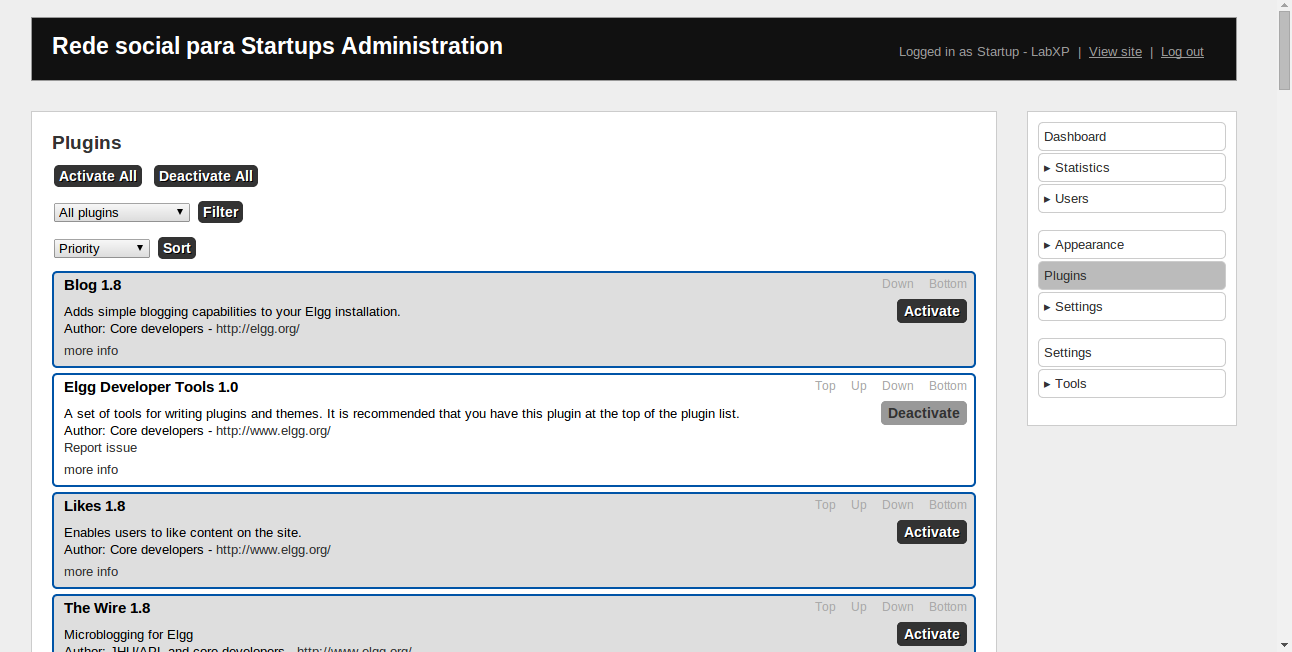
\includegraphics[scale=.35]{images/admin.png}
\caption{Janela de administrador da rede social}
\label{fig:admin}
\end{figure}


Para um melhor conhecimento do ELGG, foi colocado no diretório de Artefatos um arquivo {\bf howto.txt}, onde se encontram alguns links e informação de tópicos de desenvolvimento e configuração da rede social desenvolvida.

\section{Monashees Plus Network}
A ideia principal da rede social interna na empresa Monashees Capital, é que os membros do portfólio de empresas e principais consultores (Venture Advisors) possam trocar perguntas, respostas ideias e experiências para o desenvolvimento de todos os membros e startups que fazem parte da Monashees. \\

No primeiro protótipo da rede social se criaram e adaptaram vários plugins. Entre os Plugins desenvolvidos estão: Theme Monashees, Filters, Home, People, Venture Advisors, Sign Up Pendent List, White List, Libraries Monashees, Social Login Extend. Entre os adaptados, estão: Social Login, FirstLogin Permission, FirstLogin Redirect, Like Comment. Entre os plugins nativos utilizados estão: Search, Profile, Likes, HTMLawed.

\subsection{Plugin Filters}
O Plugin de Filter faz as principais operações de filtragem das diferentes entidades criadas por os outros plugins. Esse plugin é usado para filtrar os usuários que fazem parte da rede social, para filtrar as perguntas ou entradas feitas por os usuários no plugin do Home e para filtrar os Ventures Advisor criados pelo administrador do sistema. Veja a Figura \ref{fig:Home}.

\begin{figure}[htpb]
\centering
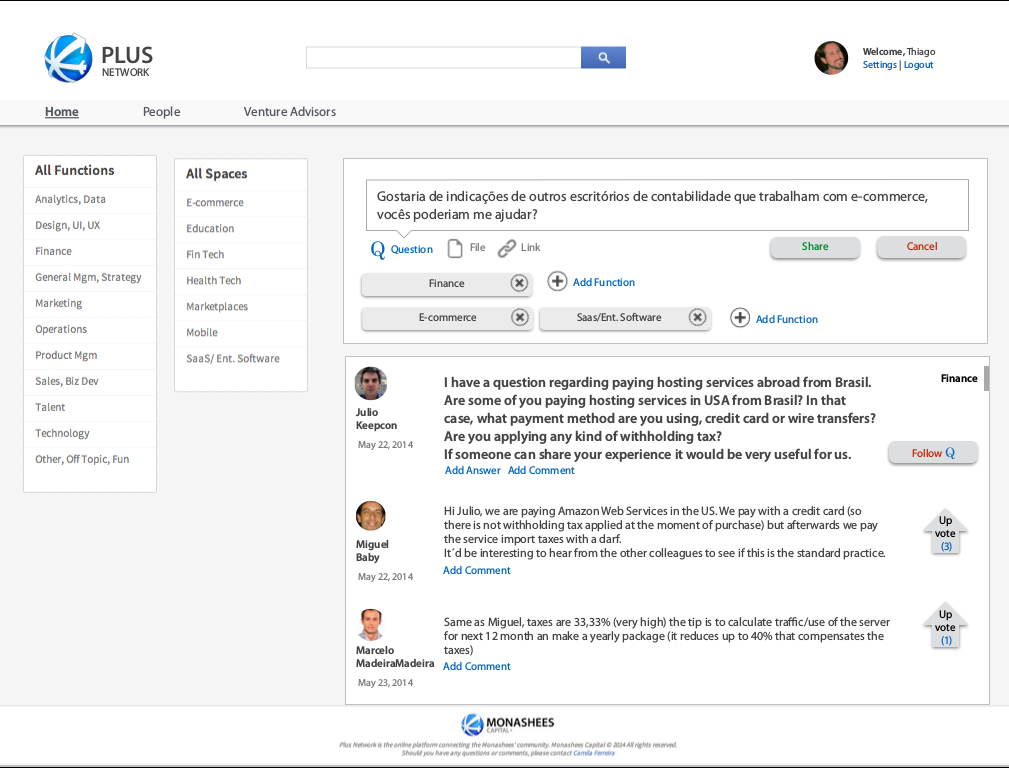
\includegraphics[scale=.35]{images/home.png}
\caption{Janela principal do plugin de Home}
\label{fig:Home}
\end{figure}

\subsection{Plugin Home}
No plugin de Home os usuários da rede social poderão submeter perguntas ou entradas ao sistemas filtrando elas por funções e espaços. Também o usuário poderá filtrar por funções e espaços as diferentes entradas que aprecem no painel principal de visualização Home.

\subsection{Plugin People}
Os usuários do sistema da rede social uma vez entram ao sistema por intermédio da rede social linkedin, terão que cadastrar as funções que ele faz no startup o empresa em que trabalham. Estes dados são requeridos uma vez entram pelo linkedin e a janela de entrada é tal como se apresenta na Figura  \ref{fig:filters}. Esta informação é usada para a filtragem de usuários no plugin de People. 

\begin{figure}[htpb]
\centering
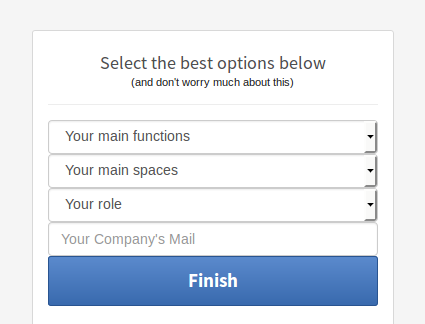
\includegraphics[scale=.5]{images/filters.png}
\caption{Janela de cadastro dos usuários da rede}
\label{fig:filters}
\end{figure}

\subsection{Plugin Ventures Advisor}
Os Ventures Advisor são colaboradores da Monashees, e eles dão apoio às diferentes startups que fazem parte do portfólio de empresas e startups. O administrador do sistema cadastra e classifica os Ventures Advisors para que os usuários da rede social possam ter acesso à informação de contato destes consultores, veja a Figura \ref{fig:VA}. ATENÇÃO: no plugin, o diretório graphic precisa estar com permissão de escrita!

\begin{figure}[htpb]
\centering
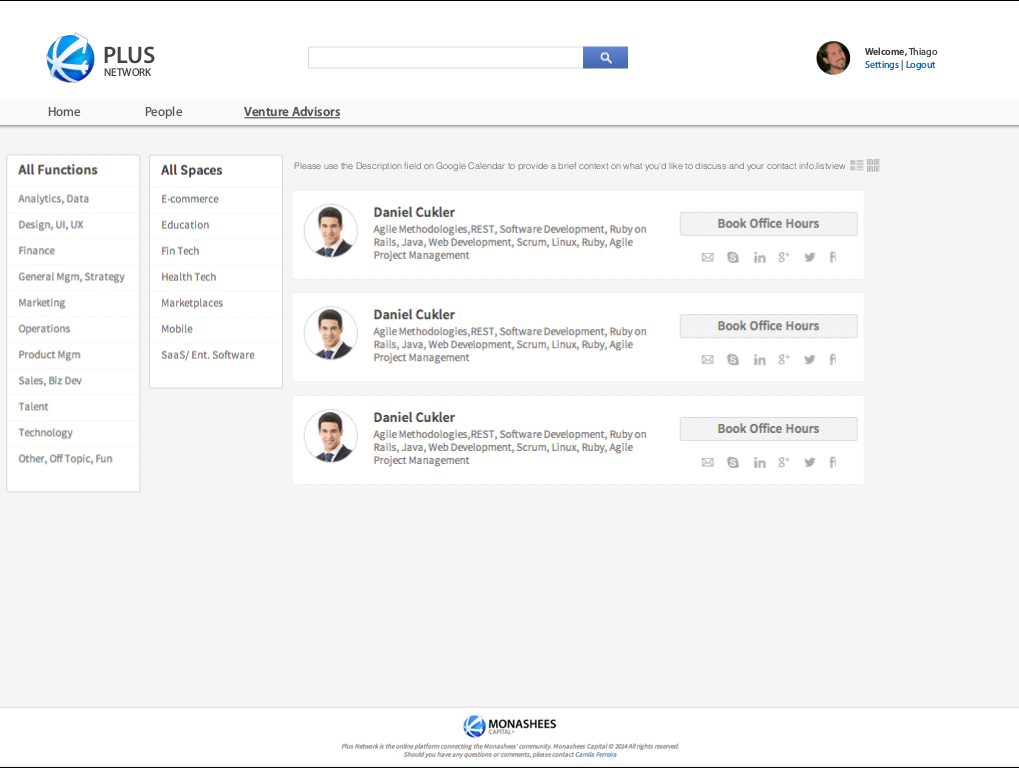
\includegraphics[scale=.325]{images/ventureAdvisor.png}
\caption{Janela de visualização de venture advisors para os usuários da rede social}
\label{fig:VA}
\end{figure}

\subsection{Plugin Theme Monashees}
O tema é visto como um plugin pelo Elgg. Theme Monashees é o plugin que personaliza as views necessárias para incorporar o layout requerido pela Monashees, seguindo os princípios de estender views ou substituí-las por completo, como é descrito na documentação. Utiliza a biblioteca Twitter Bootstrap e requer a atualização da biblioteca jQuery e do uso da biblioteca de migração, jQueryMigrate (devido a problemas de compatibilidade). O tema restrige o acesso ao site, mesmo se este estiver configurado como público. Isso permite que o plugin Social Login funcione.

\subsection{Plugin White List}
Cadastra uma White List de emails autorizados a se registrarem na Plus Network. Uma vez que o usuário esteja registrado, seu email pode ser apagado dessa lista.

\subsection{Plugin Sign Up Pendent List}
Esse plugin permite que o administrador aprove usuários que não estão cadastrados na White List de emails autorizados.

\subsection{Plugin Social Login Extend}
Estende a view do Plugin Social Login para utilizar  o botão do LinkedIn do Theme Monashees. Precisa ser o último plugin (o mais abaixo) na lista de plugins no painel do Administrador.

\subsection{Plugin Libraries Monashees}
Possui uma biblioteca que permite mudar a view de retorno de uma consulta ao banco de dados. Utilizada pelos plugins People e Sign Up Pendent List.

\subsection{Plugin Social Login}
Permite utilizar outros mecanismos de autenticação do usuário, como a API do LinkedIn, requisito do projeto. É necessário configurar os tokens do LinkedIn e precisa ter acesso público aos arquivos de autenticação. ATENÇÃO: o LinkedIn permite que testes com o domínio localhost sejam executados somente se a API estiver marcada como "em desenvolvimento". É necessário um domínio registrado para os demais casos.


\subsection{Plugin FirstLogin Permission}
Permite atribuir uma nova permissão personalizada a um novo usuário.


\subsection{Plugin FirstLogin Redirect}
Redireciona um usuário para uma página personalizada se for o primeiro login dele.


\subsection{Plugin Like Comment}
Permite dar "like" em comentários, o que o plugin nativo do Elgg não permitia pois um comentário é uma annotation e não uma entity. Precisa estar acima do Plugin Theme Monashees pois este último sobreescreve sua view, modificação seu layout.


\subsection{Formulário AfterLogin - Plugin Home}
O formulário com as informações requeridas de um novo usuário encontra-se no Plugin Home. Não é o local mais indicado mas, devido problemas técnicos, não tivemos tempo de refatorar e alocá-lo em um único plugin.

\subsection{Plugin Search}
Plugin nativo do Elgg para buscas de conteúdos. Precisa estar acima do Plugin Theme Monashees pois este último sobreescreve sua view, modificação seu layout.

\subsection{Plugin Likes}
Plugin nativo do Elgg para "likes" em conteúdos do tipo entity.

\subsection{Plugin Profile}
Plugin nativo do Elgg. Exibe o profile com as informações do usuário e, se o usuário logado for admin, permite opções como banir usuário ou apagar usuário.

\subsection{Plugin HTMLawed}
Plugin nativo do Elgg para filtrar HTML injections. Não desabilite!


\section{Testes}
O teste é muito importante no processo de desenvolvimento de um software, pois lhe garante mais qualidade, porém é uma atividade cara e demorada. Esta atividade pode inclusive consumir cerca de 50\% do total dos custos envolvidos no desenvolvimento de software. Dada a rapidez com que se queria a aplicação e o tempo gasto no aprendizagem da ferramenta foram criados testes automatizados de funcionalidades. A ferramenta para criar estes testes foi Selenium IDE\footnote{Selenium Projects - \url{http://docs.seleniumhq.org/download/http://docs.seleniumhq.org/download/}}, plugin do navegador Firefox Mozilla.

\subsection{Testes de Selenium}
Selenium IDE é um plugin do Firefox que grava e reproduz interações do usuário com o browser, veja Figura \ref{fig:Selenium}. No projeto baixado encontrará uma pasta {\texttt selenium-tests-localhost} para testes locais e {\texttt selenium-tests-nuvemusp} para testes na NuvemUSP, onde estão os arquivos de testes de funcionalidade que serão abertos com Selenium IDE. Utilize os testes para verificar as configurações dos plugins. Apenas a ordem dos plugins é necessária a verificação manual, conforme descrito no arquivo Plugin.txt em Artefatos.

\begin{figure}[htpb]
\centering
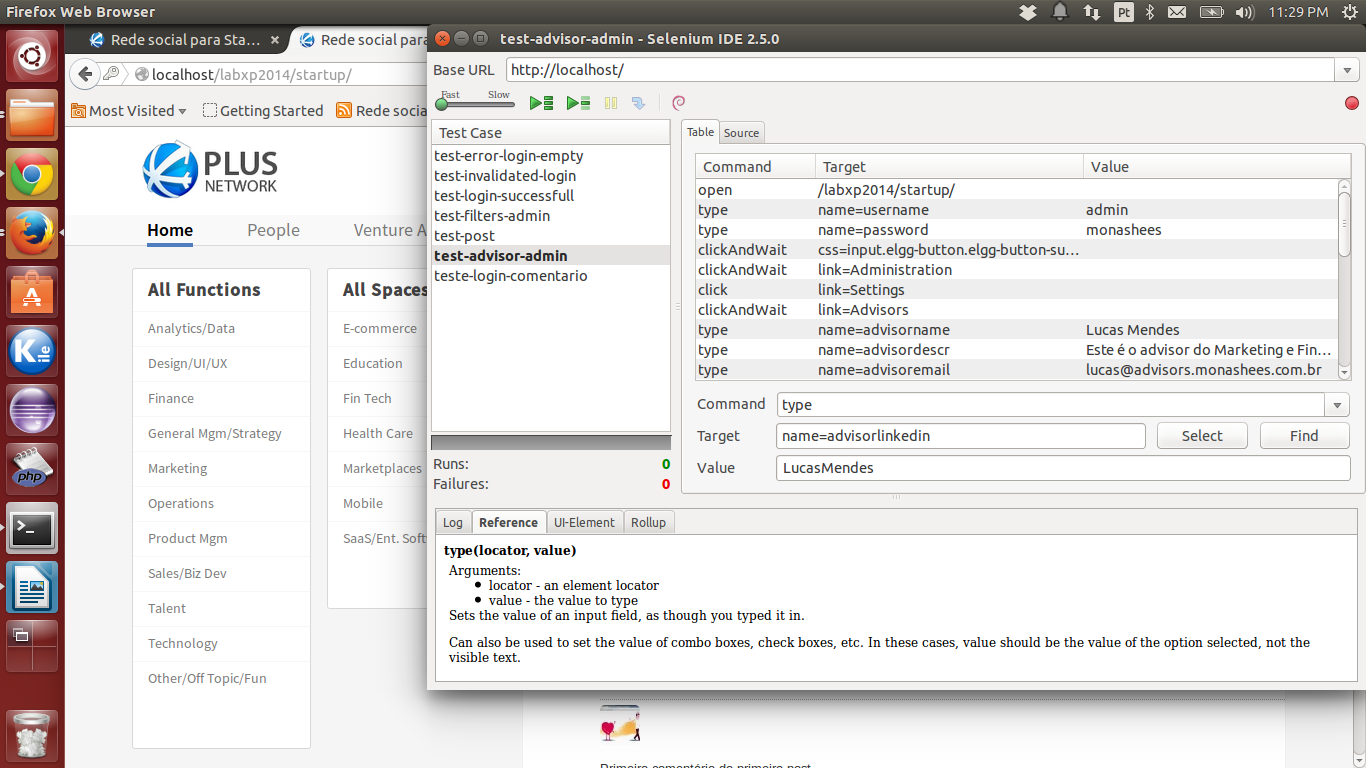
\includegraphics[scale=.325]{images/selenium.png}
\caption{Janela principal do Selenium IDE}
\label{fig:Selenium}
\end{figure}


\subsection{Testes de Unidade}

Devido a dificuldade do grupo em se adaptar a ferramenta e ao processo da disciplina por ser um projeto em estágio inicial, não foi possível estruturar os testes de unidade na ferramenta, mas é possível incorporá-los no Elgg.

\subsection{ElggUnit}

Habilitando-se o plugin Developers Tools, no menu direito aparecerá um menu Settings e, embaixo, Tools, que contém a opção Unit Tests (se o site estiver no modo debug, configurável em Advanced Settings, no campo "Debug mode provides extra information which can be used to diagnose faults. However, it can slow your system down so should only be used if you are having problems.")\\

O Elgg possui uma classe ElggCoreUnitTest para execução dos testes de unidade. Um exemplo encontrasse no plugin MyPlugin.

\subsection{PHPUnit}
Outra opção é o uso do PHPUnit\footnote{http://phpunit.de/}, que possui amplo suporte, inclusive a ferramentas como Selenium, Sonar e Jenkins.



\section{Lista de Discussões}

\url{https://groups.google.com/forum/#!forum/startup-labxp2014}

\section{Repositório Github}

\url{https://github.com/marcosamaris/labxp2014}

\section{Sonar}
É necessário instalar um plugin para que o Sonar seja capaz de analisar o código PHP. Ele analisa também testes do PHPUnit.
\url{http://200.144.254.81:9000/dashboard/index/396}


\section{Tutorial básico do Git}

\begin{itemize}
\item git clone $<$url git> : baixa um repositório
\item git status : lista arquivos locais modificados
\item git add $<$diretório ou arquivos ou . para adicionar tudo$>$
\item git commit -am "mensagem" : m é msg e a é para adicionar/excluir arquivos
\item git log : mostra commits locais
\item git pull : para baixar as atualizações do repositório; se tiver conflito, ele avisa, então você altera os arquivos listados, commita e faz o pull novamente.
\item git push remote $<$master/branch$>$ : manda para o branch que você está
\end{itemize}

Dica: \url{http://rogerdudler.github.io/git-guide/index.pt_BR.html}


\section{Sugestões}

\begin{itemize}
\item Utilizem uma VM para desenvolvimento no CEC ou notebooks. Perdemos muito tempo com problemas com o CEC (inclusive com vazamento de água!). Como utilizamos o apache, as permissões de acesso eram dadas por máquina, via chmod 777...
\item É possível utilizar o Jenkins e o PHP por meio de um template\footnote{http://jenkins-php.org/}. Esse template incorpora outras métricas de qualidade de código como detecção de copy/paste, estilo de código, dependências, entre outros.
\item Leia a documentação na internet e livros sobre o ELGG! Existe muito material sobre isso.
\item Sobre front-end, pense sempre no usuário final, que pode não ser um especialista em Elgg! Leia a documentação do W3C sobre padrões HTML, CSS e sobre acessibilidade.

\end{itemize}

\section{Contatos}

\subsection*{LabXP2014}
\begin{itemize}
\item Elaine Naomi Watanabe(coach): elaine.n.watanabe@gmail.com
\item Marcos Amaris González: marcos.amaris@gmail.com
\item Pedro Ferreira Alexandre: peferre89@gmail.com
\item Antonio Rui Sena dos Reis Castro Jr: to.junior.25@gmail.com
\end{itemize}

\section{Conclusão}
Sobre o uso do Elgg, tivemos nossas dúvidas se foi uma boa escolha durante o processo de desenvolvimento do primeiro módulo, devido ao desconhecimento da ferramenta e das próprias deficiências técnicas do grupo, uma vez que estávamos trabalhando no paradigma da web. Contudo, após o desenvolvimento de mais plugins, vimos o quanto ele era flexível e evitou conflitos no código. Um exemplo foi o uso do plugin Filters, que se integrou muito facilmente aos demais plugins. Outra vantagem foi a existência de módulos nativos como o Profile e Search, que permitiu incorporar o recurso ao sistema com o mínimo de esforço.

Sobre XP, as retrospectivas se mostraram muito importantes para identificação de problemas e resolução. Vimos também que é difícil trabalhar com um grupo com pessoas que você não conhecia inicialmente. O pareamento foi complicado em muitos momentos, mas em outros, ajudou a aumentar o engajamento da equipe (mesmo pequena dado o tamanho do projeto).

Sobre a cliente, realmente foi muito benéfico ter essa proximidade, uma vez que ela participou de todo o processo de desenvolvimento como das reuniões de retrospectiva, buscou material e contatos para nos ajudar e deu, principalmente, o feedback sobre as features implementadas rapidamente, direcionando o grupo para desenvolver recursos que agregassem valor a Plus Network.

Em resumo, na nossa última retrospectiva de encerramento do projeto, pudemos perceber que vivenciamos como é um ambiente de desenvolvimento real, como uma micro-empresa, onde foi necessário lidar com as diferenças e dificuldades do grupo (multiétnico!), negociar com o cliente (pois ele é um parceiro, faz parte do grupo!), preocupar-se com o método de trabalho em si e adaptar-se às mudanças. E, nunca esquecer, que o objetivo sempre vai ser DEIXAR O CLIENTE FELIZ! :-)


\end{document}
